
% Introduce the different experiments
% If experiment refer to each other, possibly also mention that here.

\chapter{Results \& Discussion}
The experiments performed during the project have led to many interesting results. Every experiment performed have had great impact on the AIs final performance (g: EVALUERING/ANALYS?). Either by presenting the problems and complications that the AI faces during learning or by providing a way to evaluate whether or not the modelling of the environment is sufficient.

This chapter presents and discusses the results that have been achieved during the project. The chapter is divided into sections by experiments performed. Each section presents results as well discussion and reflections about the experiments. The sections also introduce how different experiments and their results relate to each other. The order in which these results are presented follows the order in which conclusions were drawn and the project progressed (g: FOKUSERA PÅ LÄSAREN, INTE PÅ VÅRT PROJECT, TROR JAG). Thus one should get a general understanding of the AIs performance improvements during the project from this chapter.

% ----------------------------------------------------------------------------------------
% Refer to the description in method
% Present the results of the experiment
    % - What did it do?
    % - Fitness
    % - Generations required before results
    % - (Population)
% Analyse the results and the meanings behind them.
    % - Was it a good result? Why/Why not?
    % - What conclusions can be drawn from the results?
    % - How could we modify this experiment in order to get additional meaningful results?
% ----------------------------------------------------------------------------------------

% refer to the description in Method
% example: did it help to help in any way
% example: present data
% example: did the hypothesis work
\section{Constant speed}
% constant speed -> focus on steering, one variable
% gradually increasing speed, method?
% increasing speed -> push the limits 

KEY FINDINGS: INTERPRET DATA WELL, FIND COMPLEX BEHAVIOUR, NOT OBSERVED TO OPTIMISE EVERYTHING IN THE SAME SOLUTION(?), HARD TO SEPARATE SIMILAR SCENARIOS, ...

By locking the speed of the car to a constant value, conclusions about the AIs ability to steer the car could be drawn. The constant speed was gradually increased with the goal to force the AI to drive more intelligently and to find its limitations. 

Noteworthy is that after the car completes a track, rewarding it for improved time or improved distance driven is analogous. Since the car is driving at a constant speed, this will only result in a shorter distance being driven to get around the track.

The experiment was performed in two ways, one where the AI can look further down the track and one where it only has local knowledge about the track. Results for each of these sub-experiments are presented in the subsections below.

\subsection{Only local perception}
Providing the system only with local perception and giving it control of the steering, as explained in section 3.6.1, present successful and interesting results. The system immediately learns to positioning the car in the middle of the track at all times is preferable. Given that the system only has knowledge about the local relation between the car and the track, this behaviour is reasonable.

On straights this behaviour works well, it could even be considered optimal behaviour in some scenarios, however in corners it is not. When the car approaches a corner the middle of the track is shifted, causing the car to become out of position. At this point, the system tries to adjust the cars position. Before the system has had sufficient training, the amount of steering performed is either to large or to small. To large of an adjustment causes the car to oscillate between the middle line of the track, which eventually causes the car to crash. To small of an adjustment instead results in the car not getting back to the middle, eventually causing the car to crash as well. It has been observed that the oscillation occasionally helps the car to complete a complicated corner, by positioning the car in a good way. Even though this behaviour improves fitness and in theory could make the car complete the lap with a higher constant speed, the behaviour is not target behaviour. Oscillating between the middle of the track is not an optimal behaviour in racing.

The amount of training required to take a complete lap, if possible, is dependent on the constant speed of the car. At a constant speed of 10 m/s it takes approximately two generations for the car to take a complete lap. At this point the oscillation has stopped, and the car follows the middle of the track at all times. Increasing the constant speed to 11.6 m/s, causes the generations required to perform a complete lap to increases to five generations. At 11.7 m/s the generations required were 22. At these speeds, the car switches between oscillating and doing to small of a steering adjustment, causing the car to crash. When the car eventually completes a lap, there is no oscillating behaviour. Further increasing the speed, caused the car never to complete the lap. This also caused the oscillating never to stop, due to the turning radius being to small to complete a corner when sticking to the middle of the track.

[NOTE: Add network structure, what input were used in order to achieve this behaviour? Does it behave differently if we take away distance to edge/distance to middle? Size of network?]

This experiment can in general be considered a success. It was confirmed that NEAT can find behaviours that are applicable to steering a race car, and in some scenarios it can even find optimal behaviours. It is however impossible for this solution to sophistically prepare for an approaching curve. The only way for the system to determine whether or not the car should turn, is based on the current distance from the middle of the track. Which does not tell it anything about the corner in front of the car. It would be interesting to see how the system reacts to information about the upcoming part of the track. Is it possible for the system to plan ahead, in order to position the car such that it can travel through tough corners with higher speed?

\subsection{Local perception and track curvature}
\label{subsec:fixedspeedcurvature}

% Ser vi något intressant om vi ökar hastigheten
% Beteende:
% - Klarar högre hastigheter
% - Svänger före kurvorna
% - Tar mer höjd inför kurvorna
% - 

% Beteendeanalys:
% - tolkar datan bra
% - beter sig i stora delar som man kan förvänta sig
% - Begränsad av hastigheten och bilens prestanda, som vi ser när man ökar hastigheten att beteendet blir "sämre"

% Data:
% - när tar den ett varv
% - när blir det optimalt
% - storlek på nätverket och vilka indata

% Analys:
% - Vilken data användes för det här problemet/beteendet?
% - Hur lyckades NEAT hitta något
% - Kan den lära sig flera saker samtidigt?

When using the track curvature data in addition to the local perception, solutions that completed the track was found up to 12.1 m/s. It is 0.4 m/s more than was found not using the curvature data. The difference in speed may seem small, but the difference in behaviour is substantial.

What the solutions found generally do is that they position themselves well before a curve, to compensate for the larger turning radius required. They also start to steer before the curve actually start.

The speed that provided the most correctly looking race lines was 12.0 m/s. At that speed the AI had to push the limits in order to manage the toughest chicane. When the speed increased, the AI had to start turning very late in the chicane, to make a little more space for the following curve. This made it less interesting to investigate further, since that behaviour resembled real behaviour less.

% Check for longer training sessions
Each of the solutions found showed some typical characteristics. If one solution managed to drive tightly to the inner side in the toughest curve or positioned itself extremely before a curve, it also showed that tendency for all other mayor curves. On the contrary, if it turned late in the tough curves, it also did it for the other curves too.

%Check for longer training sessions
The recurrent characteristics in the behaviour for a particular solution often had one limitation, that they failed to manage simpler as efficient as the tough curves. If the solution managed to take the tough curve, near optimally, we never observed that it also managed to take the simpler curves as efficiently. For example, for the lightly turning curves, the car always drove a few meters from the edge of the track, even if it certainly had traction to stay closer. 

%Check for longer training sessions
It seemed like it did not learn to distinguish properly between the different difficulties, and simple did the same behaviour in miniature. Worth noting was that these training sessions lasted for only about 2-600 generations. We have not proven that it is not possible if one trains for longer.

OLD: The best network found for the speed 12.0 (SPEED 50????!!!?!??!!) had fitness 5821.93. It had a total of 9 hidden nodes, a total of 20 edges, 8 edges within the hidden layer, 4 to output nodes, 9 of the input nodes and bias was connected (0, 1, 3, 4, 5, 7, 8, 10, 13, 15) (bias, distance to middle, distance to right edge, angle to mid line, curve data points 10m 42m 66m 144m 397m and the segment sum of the first four points in the region 10-66m) (Remember to check which edges are enabled!)


\subsection{Shortest path}

The fastest route for a car that moves forward with a constant speed is the shortest one. This means that the only way for a genome to increase its fitness once it completes the circuit is to decrease the distance driven around the track.  

The result show that after the algorithm finds specimens that are able to complete the circuit, the gene pool continues to improve. The path around the circuit is shortened to a great extent. The difference in length of the race line and the middle line of the circuit is significant. 

The optimal behaviour is intuitively to always drive on the inner curves and to drive a straight line between the curves where it has to turn. Small variations on the curvature should not matter, if the edge does not intersect with the path the car drives.

The car follow the key behaviour aspects, but not to the extent that the path is optimal. We can see that it drives tightly to the inner side for very tight curves, but not for low intensity curves.

Training times...

Network structure...


%\section{(Existing steering controller)}
% refer to the description in Method
% example: did it help to help in any way
% example: present data
% example: did the hypothesis work

\section{Steer and speed control}
% Beteendeanalys
% - It actually does optimise for time, which is nice!
% - How does the behaviour progress? What tendencies can be seen during the training? What kind of problems does it get stuck at?
% training, data
% - It does not brake/accelerate before/after curves. Why is this? Could the input potentially be modified, such that it is easier for the system to realise what needs to be done? Distance to next curve? 
% - It stays in the middle of the track, instead of performing optimal race lines.
% - 

% Analysis
% - Can it manage to learn many components of the behaviour at the same time? One component only may make the performance worse
% - How do the behaviour / performance differ to the fixed speed. 
    % - The amount of training required is a lot higher. Compared to ~1000 generations of fixed speed, which resulted in an almost perfect race line.
    % - Its similar to fixed speed, but a little bit worse.
    

    % - Its similar to fixed speed in time during the laps, fixed speed with 12.f is a little bit faster. (Include details)
    % - When it comes to race lines, fixed speed is A LOT better. Introducing the steering/breaking output makes the performance worse in general. Why?

When the genomes are given steering and breaking as a second output, the complexity of the computations increase significantly according to the results. It takes this experiment 506 generations until a genome can complete a single lap around the track. This genome have the ability to both use the break and throttle, but still holds a lower average speed than the best genomes in the corresponding constant speed experiment.

After a genome manages to complete a lap, the data shows that the training process actually manages to find genomes that can drive faster around the track. The process of finding a genome that reaches all the way around goes much faster than the time optimisation process. As seen in figure \ref{fig:steerspeeddata} on page \pageref{fig:steerspeeddata}, the best genome of each generation increases rapidly until the fitness exceeds fitness of 5200. As this level of fitness have been reached, the training process have a gradual curve compared to the steep curve before reaching fitness of 5200. 


\begin{figure}[h]
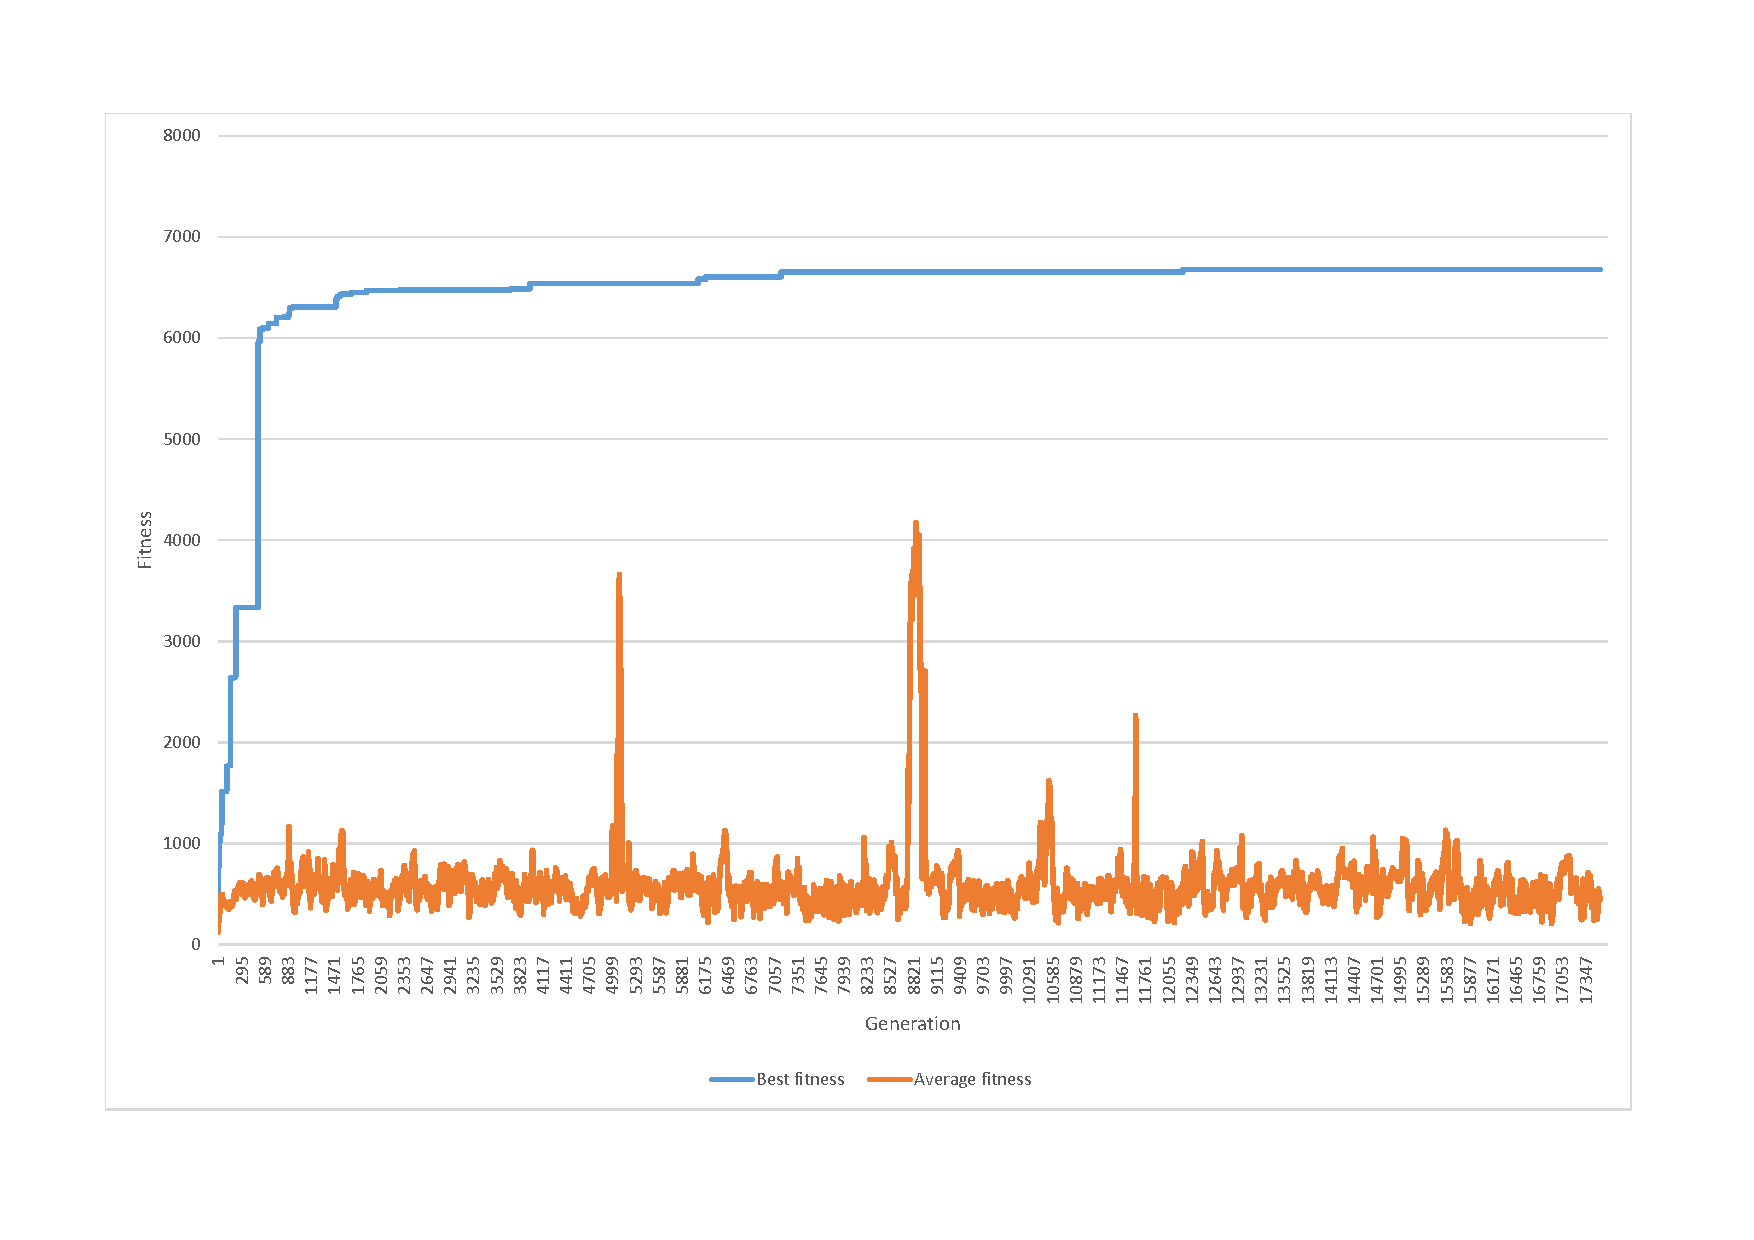
\includegraphics[width=\textwidth]{report/images/graphs/fitness}
\centering
\caption{UPDATE FIGURE! Showing best fitness and average fitness of each generation. Note that after 506 generations the fitness value surpasses 5200 as the circuit have been completed.}
\label{fig:steerspeeddata}
\end{figure}

When comparing the data in figure \ref{fig:steerspeeddata} on page \pageref{fig:steerspeeddata} to the results in subsection \ref{subsec:fixedspeedcurvature}; the fitness of the genomes that are able to accelerate and decelerate does not surpass the best genome with constant speed until generation 488. A higher fitness is reached in this experiment, but at the cost of more complexity.


\begin{figure}[h]
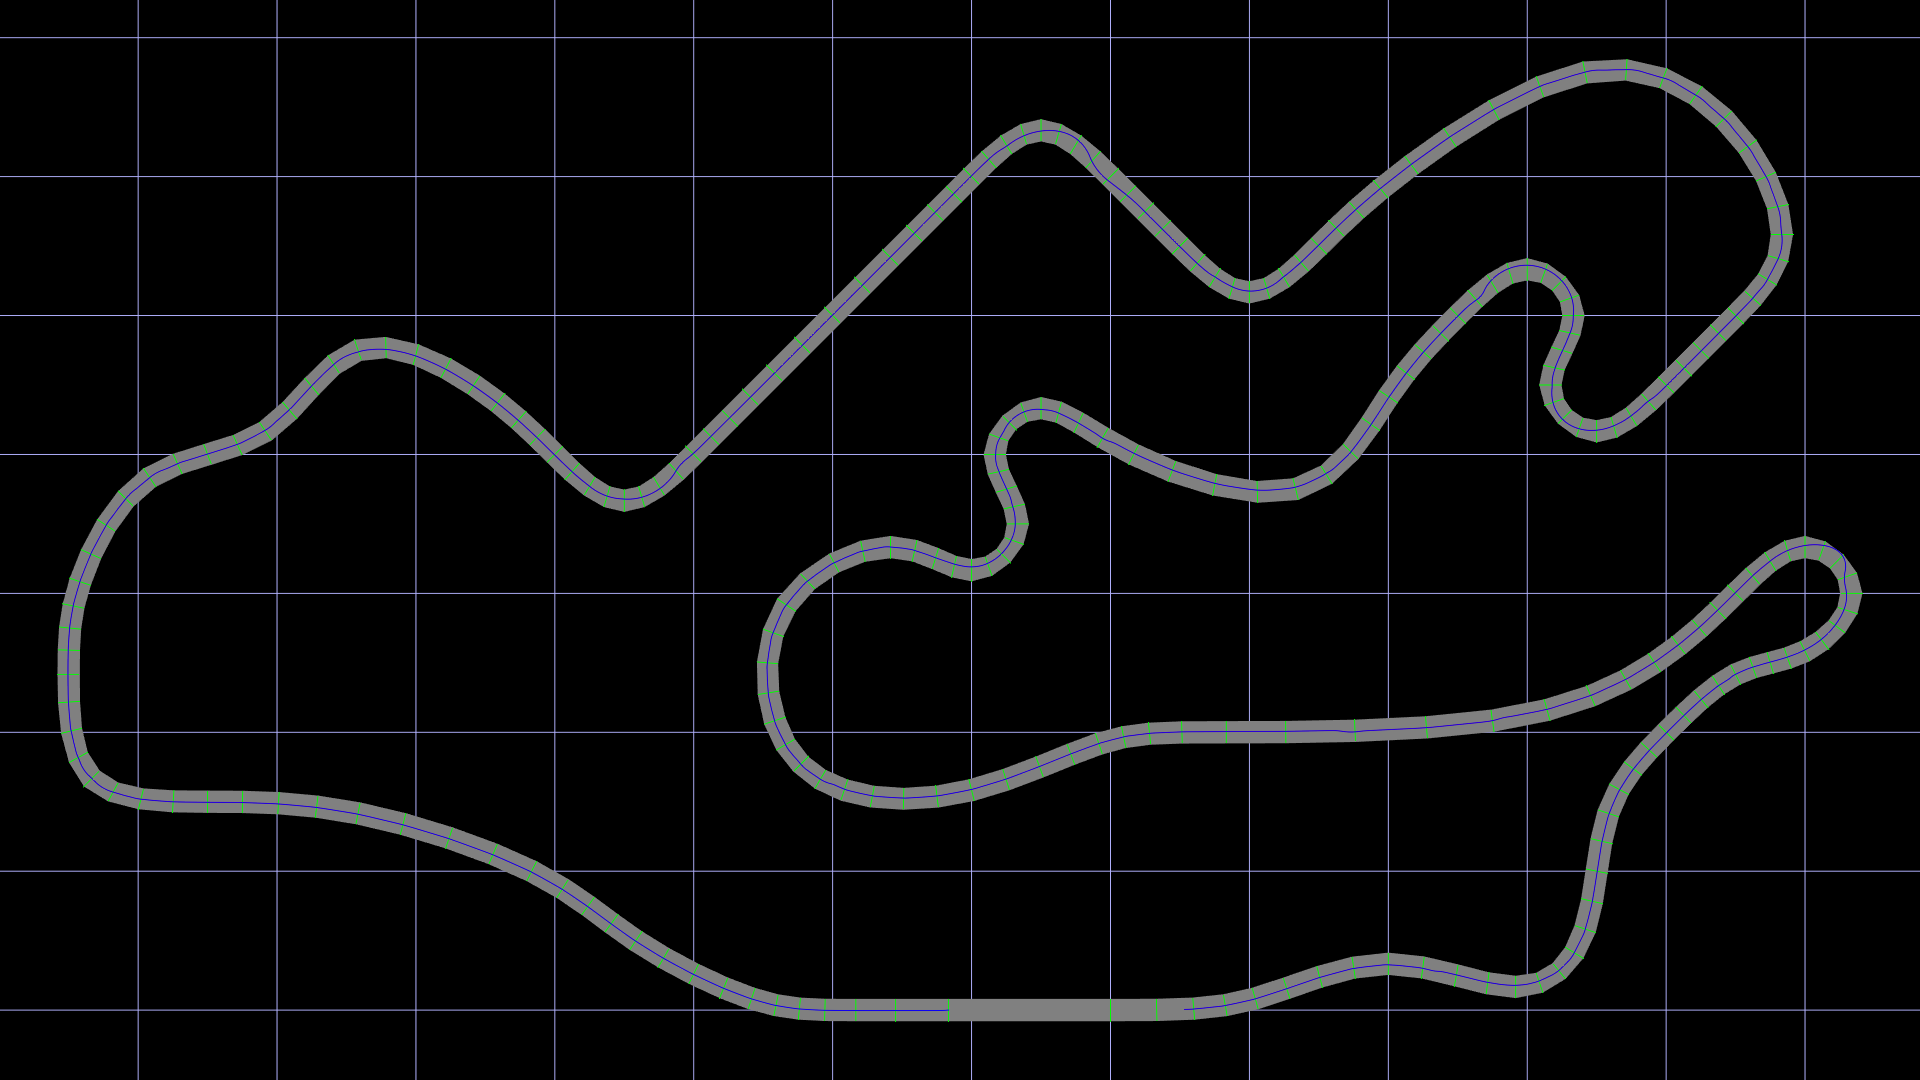
\includegraphics[width=\textwidth]{report/images/normal_generation_6558}
\centering
\caption{Showing a clockwise race line completed by a genome with a fitness value of 6587.56, the best fitness reached in the steer and speed control experiment. The speed of the car is presented by the line colour, with blue as slowest possible speed and red as max speed.}
\label{fig:steerspeedline}
\end{figure}

\section{Single short track segment}

As hypothesised in section $3.6.3$, the system is able to find more effective behaviours on shorter tracks than on the complete circuit. The behaviours found of the three track segments are not perfect, however they show signs of effective speed management, which is one of the criteria looked for the in the behaviour. The genomes do no show any significant signs of effective positioning, which is the other major criteria. 

In each experiment the most successful genomes keep a high speed until braking before the corner and accelerate out of the corner, keeping a high speed until the end of the track. 

%% Sätt in bilder där man visar inbromsningar etc. 

Even though the system did not find any near perfect behaviours, the results show that the system has a greater ability to optimise for time when training on shorter tracks. One plausible reason behind this is as mentioned in section $3.6.3$ that it is too hard to change the behaviour of the genomes are able to complete the circuit. In order change from a cautious behaviour to a more effective one the genome must learn to accelerate on straights and brake before corners at the same time. Changing only one aspect at a time will most likely lead to a worse behaviour. If a genome is changed to accelerating more it will likely crash in a sharp corner. Likewise if a genome is changed to braking before corners without accelerating more it will drive slower and thus decrease in fitness.  

\section{Multiple short track segments}

%%% KÖTTA UT


\section{Mirror track}
% TODO: Sätt in grafer och skit.

The experiment where the training environment was exchanged to a mirrored version of the same track showed several interesting results. The test population was trained on the normal circuit until the best specimens managed to complete the circuit in approximately $500$ seconds, which took $3527$ generations with a population of $500$ genomes. That population was then transferred to training on the mirrored track. On the first try, some specimens managed to complete $1800$ metres of the circuit which is about a third of the way. This shows that at least some of the genomes had some general knowledge about how to drive. However in the next few generations the population managed to complete the whole circuit. This is much faster than the control population which took approximately $150$ generations to complete the circuit. 


\begin{figure}[H]
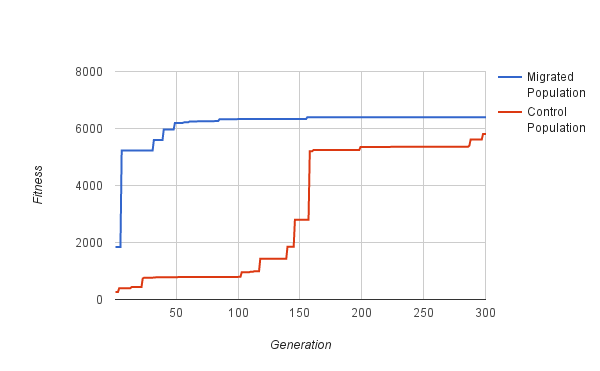
\includegraphics[width=\textwidth]{report/images/graphs/mirror_migration}
\centering
\caption{Showing the fitness progression of the migrated population shown in blue and the control population shown in red. Note that the migrated population in a few generations surpasses a fitness-value of 5000 as a result of completing the circuit. . }
\label{fig:mirrordata}
\end{figure}

This shows that some of the knowledge acquired on the first track is applicable on the second. Whether the genomes complete some corners because there are similar ones on the first track or because ... If this is the case, one could argue that in order to find a generalised behaviour the AI should train in an environment where it encounters every possible type of situation, i.e. every type of corner and combination of consecutive corners. 

% Skriv om bajsiga meningar.
The extension to the experiment where the migrated population was migrated back to the original circuit once it had adapted also showed interesting results. The population forgets knowledge when adapting to the new environment. This is somewhat expected since the population mutated for 500 generations on the mirrored track, ergo no genomes trained on the original circuit remain in the population. However not all of the knowledge is lost in the process, some generalised knowledge remain. When migrated back to the original track, one specimen manages to stay on the track for circa $2800$ metres, which is slightly past halfway around. After only $5$ generations of adapting back to the original track one specimen manages to complete the circuit, albeit slowly. The adaption to the original circuit is similar in nature to the adaption from the original to the mirrored one. 


%- If it is trained for certain tracks, can it manage others

\section{Summary of results}





% Discussion of the behaviour
% Present current results
% This chapter presents and discusses the results that have been achieved during the course of the project. We successfully present the car driving around the track. However the lap that is taken by the car is neither optimal in respect to the race lines nor the time that it takes for the car to travel around the track.

% The experiments performed during the course of the project have given varying results. Every experiment have had a large impact on how the project has progressed and on the final results. The results for each experiment and the conclusions that could be drawn are presented and discussed in this chapter.

% \section{Experiments}
% Introduce this section somehow.

% \subsection{Curve Data as input}
% Present and discuss what results this method achieved for us.
% What kind of machine learning techniques did we use? What did they do differently?
% What behaviour did we see? Why is that?
% Is this behaviour similar or identical to a real race-car driver?
% Is it the most optimal route around the track, with regards to lap time?
% Can we expand this solution further? If so, how?

% This experiment was the first one that was carried out with any real progress towards the goal. We managed to produce a machine learning algorithm efficient enough to drive the car around the track without crashing, however given some simplifications; The car automatically accelerates in a straight line, up to a certain point where it stops accelerating and keeps the same constant speed. The neural network has the possibility of controlling the amount of breaking and turning the car does, overriding any automatic acceleration that the car does by itself.

% This results in a neural network successfully driving the car around the track. However the path taken is not the optimal one. The path starts of by oscillating left and right between the middle of the track. After a few generations of training, the neural network starts to adjust the oscillating such that the sharper curves can be taken with a wider radius. Given even more training the oscillating almost disappears completely, it only remains before and after some curves.

% This behaviour is as mentioned of course not optimal, and neither is it one that a human race-car driver would chose to take. It is both longer and more complicated than would be required for simply driving around the track, without optimising for maximal speed or time.

% The training algorithm seems to converge towards a simple neural network between all of the training sessions that has been performed. The neural network produced is one with only one connection between an input and an output. The training required in order to make a complete lap, takes no more than a few minutes. These factors leads us to believe that we can increase the complexity quite significantly before the search space has become to large to be solved within a reasonable time. Thus the limit of NEAT with respect to our problem has not been reached yet.